\chapter{Актуальность исследований технологического процесса электростатического соединения кремния со~стеклом}

Проанализированы данные литературных источников за~предшествующие 45~лет по~технологиям герметичного соединения, применяемым при изготовлении электронных приборов.
Представлен обзор современных технологий, определены их~достоинства и~недостатки. Углублённо рассмотрена технология электростатического соединения кремния со~стеклом.

В~связи с~этим поставлена цель "--- изучить возможности снижения
остаточных напряжений в~сборках, вызванных разницей
в~термомеханических свойствах кремния и~стекла, соединённых анодной
посадкой.  Для достижения этой цели определены задачи по~поиску более
точных способов оценки таких напряжений и~поиску конструктивных
и~технологических решений по~их~снижению, включая подбор марки стекла.

\section{Сравнение способов соединения с~деталями из~кремния}

Микроэлектромеханические системы (МЭМС) "--- это микроминиатюрные интегральные устройства или системы, в~которых комбинируются механические и~электрические компоненты. Они изготовляются на~основе групповой технологии обработки интегральных схем и~могут иметь размеры от~нескольких микрометров до~нескольких миллиметров. Общим методом создания многослойных объёмных микромеханических устройств является соединение двух пластин~\cites[122]{Raspopov_micromechanics2007}.

Выбор подходящего метода соединения определяется рядом факторов, учитывающих, в том числе, тип (например, оптические или механические приборы) и назначение (например, коммутационные или измерительные приборы) изготавливаемого устройства; требования, предъявляемые принципом работы устройства (например, наличие герметичного шва), а также различия в свойствах материалов деталей и узлов, входящих в состав прибора (например, различающимися коэффициентами теплового расширения)~\cite{New_low_temperature_bonding_tech,Vacuum_Packaging_Technology_and_Appl}.

Соединение, сохраняющее герметичность в~течение всего срока жизни прибора, важно для приборов, функционирование которых зависит от~неизменности параметров среды внутри них, например, работающих в~агрессивной среде~\cite{lit_harpster2002long}. Кроме того, давление внутри прибора определяет характеристики демпфирования и~амплитудно-частотные характеристики рабочих движущихся элементов таких приборов, как микроакселерометры, высокочувствительные МЭМС-гироскопы, высокочастотные резонаторы.

Соединение деталей прибора может использоваться как метод поддержания чистоты внутри собираемого устройства. Например, подложки могут быть соединены перед резкой для предупреждения повреждения хрупких или чувствительных элементов~\cite{lit_Esashi_Wafer2008}.

При выборе способа соединения следует также учитывать температурные ограничения. Это касается как ограничений по~допустимой температуре нагрева металлизации соединяемых деталей (440~{\textdegree}C для алюминиевой металлизации), так и~ограничений, связанных с~разностью коэффициентов температурного расширения.

Также следует учитывать накладываемые способом соединения ограничения
на~возможность создания электрических соединений между деталями
в~сборке. Присутствие свинца (соединение стеклоспаями), натрия
(анодная посадка) или золота (эвтектическое соединение) должно быть
учтено, если одна из~соединяемых деталей содержит полупроводниковые
структуры~\cite{Dragoi_cmos_wafer_bonding}.

В~Таблице~\ref{tab:compare_bonding_methods} приведено сравнение способов соединения с~точки зрения различных требований с~учётом описанных выше ограничений~\cite{New_low_temperature_bonding_tech,Dragoi_cmos_wafer_bonding,Babaevskij_korpusirovanie_NMST2014_3}.

\begin{table} [!bh]%Порядок, в котором заданы опции, позволяющие регулировать положение рисунка на странице, не важен — они всегда будут применяться в порядке h (здесь) — t (вверху) — b (внизу) — p (на отдельной странице). Важно только то, какие именно опции заданы. По умолчанию — [tbp]. Задавать опции по одной (например, просто [t] или просто [b]) не рекомендуется — в некоторых случаях это может приводить к проблемным ситуациям.
	\caption{Сравнение способов соединения}%
	\label{tab:compare_bonding_methods}% label всегда желательно идти после caption
    \renewcommand{\arraystretch}{1.3}%% Увеличение расстояния между рядами, для улучшения восприятия.
	\def\tabularxcolumn#1{m{#1}}
	\newlength{\tabcellen}
	\setlength{\tabcellen}{\widthof{соединение}} %
	\begin{SingleSpace}
	\begin{tabularx}{\textwidth}{@{}
	>{\raggedright}X
	>{\centering}m{1.9cm}
	>{\centering}m{1.9cm}
	>{\centering}m{2.0cm}
	>{\centering\arraybackslash}m{1.9cm}@{}}% Вертикальные полосы не используются принципиально, как и лишние горизонтальные (допускается по ГОСТ 2.105 пункт 4.4.5) % @{} позволяет прижиматься к краям
        \toprule     %%% верхняя линейка
    	Критерии сравнения (требования к~процессу) & Анодная посадка &
    	Стекло\-сплав &
    	Эвтекти\-ческое соединение &
    	Прямое сращивание	\\
        \midrule %%% тонкий разделитель. Отделяет названия столбцов. Обязателен по ГОСТ 2.105 пункт 4.4.5
        Совместимость с~КМОП &
        ${\pm}$ &
        ${\pm}$ &
        ${\pm}$ &
        $ + $ \\
        Температура процесса {\textless}440~{\textdegree}C &
        $ + $ &
        $ + $ &
        $ + $ &
        $ - $ \\
        Отсутствие требования механического прижатия &
        $ + $ &
        $ - $ &
        $ - $ &
        ${\pm}$ \\
        Отсутствие требований к~равномерности прижатия &
        $ + $ &
        $ - $ &
        ${\pm}$ &
        $ - $ \\
        Герметичность соединения &
        $ + $ &
        $ + $ &
        $ + $ &
        $ + $ \\
        Возможность формировать вертикальные электрические межсоединения  &
        $ + $ &
        $ - $ &
        $ + $ &
        $ + $ \\
        Допустимая высота выступов на~поверхности, не~более, мкм &
        0,05 &
        2 &
        1 &
        0,004  \\
        \midrule%%% тонкий разделитель
        \multicolumn{5}{@{}p{\textwidth}}{
            \vspace*{-4ex}\hspace*{2.5em}Примечание "---  <<$+$>> "--- требование полностью выполняется; <<$-$>> "--- требование невыполнимо; <<${\pm}$>> "--- требование выполняется в~некоторой степени с~ограничениями или особенными условиями соединения.
        }
        \\
        \bottomrule %%% нижняя линейка
	\end{tabularx}%
	\end{SingleSpace}
\end{table}

\subsection{Прямое сращивание}
Прямое сращивание пластин это технология соединения двух кремниевых
пластин без приложения электрического напряжения, обычно при комнатной
температуре. Прямое сращивание также называют соединением методом
сплавления кремния~\cites[123]{Raspopov_micromechanics2007}.
Данный процесс основывается на~химической реакции между группами ОН\textsuperscript{\(-\)} или H\textsuperscript{\(+\)}, находящимися на~поверхности исходного кремния или на~образованном на~подложке слое оксида кремния~\cites[487]{lit_madou2002fundamentals}. Прямое сращивание обычно состоит из~трёх этапов: подготовки поверхностей, соединения поверхностей и~термической обработки. Подложки с~высоким качеством полировки после химической обработки предварительно соединяются, выравниваются и~довольно сильно сжимаются в~центральной точке поверхности. Шероховатость соединяемых поверхностей подложек не~должна превышать 4~нм~\cites[487]{lit_madou2002fundamentals}. Неплоскостность пластины не~должна превышать 5~мкм (для пластин диаметром 100 мм)~\cite{schmidt1998wafer}. Соприкосновение двух гидрооксидных плёнок на~подложках приводит к~установлению плотного контакта по~всей поверхности кремниевых пластин. Последующая термообработка проводится при температуре 1100~{\textdegree}C и~создаёт долговременные ковалентные связи~\cite{stoger1999awbtech}. При более тщательной подготовке соединяемых поверхностей температуру термообработки можно понизить до~400~{\textdegree}C~\cite{lit_resnik2000study}.

\subsection{Эвтектическое соединение}
Эвтектика "--- жидкая система (раствор или расплав), находящаяся при данном давлении в~равновесии с~твёрдыми фазами, число которых равно числу компонентов системы~\cite{bse_eutectic}.
Добавляя или отводя тепло, можно изменить пропорцию между кристаллическими фазами и~расплавом в~эвтектической точке без изменения температуры~\cite{wiki_eutectic}.

<<Эвтектика является пересечением поверхностей равновесия расплава с~соответствующими (эвтектическими) фазами. Если отводится соответствующее количество тепла, то~расплав эвтектического состава при кристаллизации в~условиях близких к~равновесным даст все кристаллические фазы, участвующие в~равновесии. Если же~подводится тепло в~достаточном количестве, то~смесь фаз, отвечающая эвтектическому составу, в~условиях близких к~равновесным будет плавиться с~одновременным уменьшением доли каждой из~кристаллических фаз вплоть до~их полного исчезновения>>~\cite{wiki_eutectic}.

Эвтектическое соединение широко распространено в~микроэлектронной
промышленности.
Его применяют как для посадки кристаллов интегральных схем и~дискретных приборов
в~металлокерамические корпуса, так и~для соединения кристаллов
микроэлектромеханических приборов с~подложкой.
Соединяемые материалы нагревают до~температуры эвтектической точки, при которой
начинается процесс взаимодиффузии металлов, входящих в~эвтектический
сплав~\cite{Dragoi_cmos_wafer_bonding}.
После охлаждения сборки получают прочное и~надёжное соединение деталей.
Температура эвтектической точки для системы кремний"--~золото составляет
370~{\textdegree}C~\cites[396]{Ljakishev1996_diag_dvojnyh_met_sis_t1}, для
системы алюминий"--~германий составляет
424~{\textdegree}C~\cites[152]{Ljakishev1996_diag_dvojnyh_met_sis_t1}.

Проблемой эвтектического соединения является получение равномерного прочного соединения больших поверхностей. Даже естественные окислы мешают образованию соединения. Процесс проведения эвтектического соединения требует приложения значительных усилий. Следствием этого является сложность соединения деталей большой площади, так как кроме обеспечения прижима необходимо обеспечить высокую степень чистоты и~равномерности соединяемых поверхностей.

\subsection{Соединение стеклосплавом}
Соединение стеклосплавом проводится следующим образом. Паста, полученная в~результате смешивания порошкообразных минералов с~растворителями, наносится на~одну из~соединяемых деталей и, затем, тщательно высушивается. После этого, пластины соединяют при температуре большей, чем точка размягчения высушенной пасты. Типовая температура процесса находится в~диапазоне от~400~{\textdegree}C до~600~{\textdegree}C~\cite{stoger1999awbtech}. Для получения высококачественного соединения необходимо равномерное приложение механического усилия.

\subsection{Электростатическое соединение}
<<В 1960 г. Н. А. Иофис предложил повышать прочность пайки керамики с~керамикой и стекла с металлом воздействием внешних электрополей~\cite{iofis_patent1960}. Особенно бурное развитие исследований, посвящённых разработке методов сцепления твёрдых тел под воздействием внешних электрических полей, начинается с 1967~г., когда в СССР
и США~\cite{AB_patent_Pomerantz_1968} вышли первые публикации по указанной проблеме. Появилась возможность создавать как обратимый адгезионный контакт, сохраняющийся только при действии внешнего электрического поля, так и необратимый>>~\cite{evdokimov_krestov1988}.

Электростатическое соединение "--- это технология герметичного соединения стекла с~высоким содержанием окислов щелочных металлов с~металлом или полупроводником при повышенной температуре и~приложенном высоком напряжении. Будучи изначально разработанной для соединения стекла с~металлами~\cite{AB_patent_Pomerantz_1968}, данная технология получила широкое распространение в~микроэлектронике для соединения кремния со~стеклом~\cite{New_low_temperature_bonding_tech,lit_Esashi_Wafer2008,ushkov_kozlov2007}.

<<В~русскоязычной литературе этот процесс имеет также следующие названия:
анодная посадка, анодное сращивание>>~\cite{Sinev_technomag2014},
анодное соединение~\cites[122]{Raspopov_micromechanics2007},
термоэлектростимулированное соединение, электростимулированное термическое соединение~\cite{timoshenkov2006issledovanija},
<<электростатическая сварка~\cite{andreev2014kremnievye}, электроадгезионное соединение, электродиффузионная сварка>>~\cite{Sinev_technomag2014},
неуправляемый электроадгезионный контакт~\cite{tonkiy1974eak_avtoref}, электрохимическая сварка в~твёрдой фазе~\cite{khomenko2001proizvodstvo}, сварка в~электростатическом поле~\cite{berezin2001}.

В~англоязычной литературе устоялись следующие синонимичные названия этого процесса: anodic bonding, field assisted bonding, field-assisted thermal bonding, electrostatic bonding, Mallory process, electrostatic welding~\cites[484]{lit_madou2002fundamentals}.

Процесс электростатического соединения проводится при температуре от~180 до~500~{\textdegree}C как на~воздухе, так и~в вакууме~\cites[484]{lit_madou2002fundamentals}. Электростатическое притяжение между стеклом и~кремнием исключает необходимость приложения значительного усилия к~соединяемым подложкам в~процессе соединения.

Кремниевую пластину помещают на~стеклянную пластину. Соединяемые
поверхности нагревают. Отрицательный электрод источника высокого напряжения
 прикладывают к~стеклянной пластине, а~положительный электрод "---
к~кремниевой пластине. Значение прикладываемого напряжения составляет от~200
до~1500~В~\cites[484]{lit_madou2002fundamentals}{Khomenko1982useglassproperties, Khomenko1990physprocess}. Процесс в~среднем проходит за~30~минут.

В~отличие от~управляемого электроадгезионного контакта, основанного на~эффекте электростатического притяжения Джонсона"--~Раббека~\cite{johnsen1923physical,atkinson1969simple}, при анодной посадке отведение потенциала не~разрушает уже сформировавшееся соединение~\cite{evdokimov1968issledovanie_avtoref}.

К преимуществам технологии анодной посадки относят:
\begin{enumerate}
    \renewcommand{\labelenumi}{\asbuk{enumi})}
    \item относительно низкую температуру процесса, поэтому нет опасности разрушения
    металлических слоёв (например, алюминиевых)~\cite{Low_temp_wafer_AB}, входящих
    в~состав элементов микросхем;
    \item герметичность соединения и возможность её сохранения при использовании с
    технологиями формирования электрических межсоединений сквозь стекло или
    кремний~\cite{lee_rogers2011ssi_design_rules_wlp};
    \item использование оптически прозрачного стекла, что облегчает процесс
    совмещения соединяемых пластин, а также может быть важным для оптических
    приборов~\cite{shoji1998low_b_quartz};
    \item применение стекла позволяет снижать паразитные ёмкости у чувствительных
    элементов датчиков, работающих на емкостном принципе, а~в~электростатических
    системах полезны диэлектрические свойства стекла~\cite{shoji1998low_b_quartz}.
\end{enumerate}

Недостатком технологии считают возможность выделения кислорода из~стекла
в закрытые полости в процессе проведения соединения кремния
со~стеклом~\cites{lit_Esashi_Wafer2008,lee_rogers2011ssi_design_rules_wlp}[С.~3-20]{gad2006mems_applications}{barinov2015_datchik_zhestk,Rogers1992considerations,timoshenkov2010metody}.
%NEEDFIX неправильная длина тире в интервале страниц в ссылке на источники, но залитый в ВАК диссер изменять нельзя, так что это не подлежит исправлению в исходниках моей диссертации

\section{Подробное рассмотрение технологии электростатического соединения}

\subsection{Обзор применений процесса}

Электростатическое соединение применяют при изготовлении чувствительных элементов датчиков давления~\cite{kozin2010_microel_datch_fiz_vel}, а также разнообразных приборов электронной техники, таких как микрорезонаторы, микрореле, микроакселерометры~\cite{lit_Esashi_Wafer2008}, микрогироскопы~\cite{Rogers_current_limited_AB_2005}. Эту технологию применяют при герметизации оптических приборов, например инфракрасных датчиков~\cite{lit_Esashi_Wafer2008}, а~также для интеграции микромеханических систем с~оптическими~\cite{saran2003_ab_opt_fibers}. В ряде случаев соединяют полированные поверхности без топологии, например, при изготовлении чувствительных элементов датчиков давления~\cite{Andreev2013_Analiz_met_elektrostat_svar}. Возрастающая сложность приборов обуславливает необходимость соединения деталей, поверхности которых уже обработаны и покрыты плёнками различных материалов~\cite{Dragoi_cmos_wafer_bonding}.

Соединяют как отдельные кристаллы стекла и кремния, так и целые пластины. Соединение пластин предпочтительней, потому что оно обеспечивает более точное совмещение. Для получения качественного соединения необходимо обеспечить ряд требований~\cite{Low_temp_wafer_AB, Cozma_Puers_1995, Sinev_osoben_primen_inzh_vest201408}:
\begin{enumerate}[label=\asbuk*)]
    \item качество соединяемых поверхностей должно быть высоким (следует обеспечить
    низкую шероховатость и высокую чистоту поверхностей); %NEEDFIX «низкую шероховатость и высокую чистоту поверхностей» = стилистическая ошибка по мнению ведущей организации, но залитый в ВАК диссер изменять нельзя, так что это не подлежит исправлению в исходниках моей диссертации
    \item температура процесса должна быть достаточной для обеспечения
    подвижности ионов, и, одновременно, достаточно низкой, чтобы
    не~ухудшить характеристики создаваемого прибора;
    \item распределение температуры и подводимого заряда по
    поверхности должно быть равномерным;
    \item коэффициенты теплового расширения соединяемых материалов
    должны быть согласованы;
    \item число подвижных ионов в стекле при рабочей температуре
    должно быть достаточным для проведения процесса.
\end{enumerate}

\subsection{Основные соединяемые материалы и~критерий их~выбора}
\begingroup
Процесс электростатического соединения может быть применён для
соединения стекла с металлами, сплавами и полупроводниковыми
материалами~\cite{wallis_pomerantz1969fagms}. Практически этот процесс
распространён на боросиликатные, алюмосиликатные, щелочные и
оптические стекла, а так же на керамические
соединения~\cite{wallis_pomerantz1969fagms}. Стекло с достаточно
большим коэффициентом содержания щелочных металлов может быть
соединено с полупроводниками (Si, Ge,
GaAs)~\cite{wallis_pomerantz1969fagms,
Khomenko1996pyrex}, с~металлами и~сплавами (например, Al, Cr, Wo, Ta,
Ti, ковар)~\cite{Khandan2014titanium_ab}
и~с~полупроводниковыми структурами (такими как SiC,
Si\textsubscript{3}N\textsubscript{4}, SiO\textsubscript{2})
\cite{stoger1999awbtech}. Толщина слоя изолирующего материала, такого
как SiO\textsubscript{2}, должна быть минимальна (на уровне
естественного окисла), чтобы пропустить достаточный
ток~\cite{stoger1999awbtech}.
В~работе~\cite{djachkov2000_avtoref} проведено исследование влияния состава ряда отечественных стёкол (включая ЛК105 и~К8) на~плотность тока при сращивании с кремнием.\russianpar
\endgroup

Важным критерием при выборе пары соединяемых материалов является их согласование по значению ТКЛР.

Идея электростатического соединения стекла и кремния может быть заимствована и для соединения кремния с кремнием. Одна кремниевая поверхность с тонкой стеклянной плёнкой будет катодом. Минимальная толщина стекла для удовлетворительного соединения "--- 4 мкм~\cites[487]{lit_madou2002fundamentals}{Wallis_FAGS_1975}. Напряжение необходимое для сращивания составляет 50~В~\cite{Wallis_FAGS_1975}.

Стеклянные пластины могут быть соединены электростатическим сращиванием через слой кремния. На одну из стеклянных пластин наносят тонкую плёнку кремния, через которую будет проходить соединение с другой стеклянной пластиной~\cite{terazaki2012stack_structure_patent}.

\subsection{Требования к~качеству соединяемых поверхностей и~давлению в~камере}
Прочное соединение при электростатическом соединении достигается при хорошо обработанных поверхностях обоих соединяемых объектов~\cite{Wallis_FAGS_1975}. Шероховатость поверхности с целью получения наиболее прочного соединения должна быть не более Ra\,1,0~мкм~\cites[484]{lit_madou2002fundamentals}.
При увеличении шероховатости необходимо повышать температуру нагрева, электрическое напряжение и время выдержки.

Степень очистки поверхности перед посадкой также влияет на качество
соединения. Например,  очистка раствором
H\textsubscript{2}SO\textsubscript{4}–H\textsubscript{2}O\textsubscript{2}
и HF обеспечивает более качественную посадку~\cite{Lee_Detailed_characterization},
чем очистка ацетоном.
Ацетон используется, чтобы смыть нерастворимые и свободно лежащие органические остатки,
но~не~в~состоянии удалять окись и другие следы загрязнений на поверхности,
которые затрудняют процесс посадки.

Также поверхности перед посадкой при необходимости активируют плазмой~\cite{choi2002analysis} различного газового состава, которая может удалять и естественный окисел.

Чем выше температура проведения процесса, тем меньшее влияние оказывает предварительная очистка поверхностей~\cite{Cozma_Puers_1995}.

Требования к составу окружающей среды определяются, как правило, требованиями к конкретному прибору или к атмосфере, герметизируемой в~приборе. Кроме того, в работе~\cite{Cozma_Puers_1995} показано, что кислород из окружающей среды повышает прочность соединения стекло"--~стекло.

\subsection{Описание процесса электростатического соединения}
При анодной посадке кремния на стекло отрицательный заряд подводится к стеклу, а
положительный "--- к кремнию (см. Рисунок \ref{fig:AB_proc_scheme}). Процесс
соединения происходит следующим
образом~\cite{Khomenko1990physprocess, Lee_Detailed_characterization, enikov2006introduction}:
при повышенной температуре и наличии сильного электрического поля положительные
ионы натрия (Na\textsuperscript{$+$}) в стекле дрейфуют к отрицательному
электроду на стеклянной пластине и нейтрализуются. Из-за их перемещения на
границе с кремнием образуется избыточный отрицательный
заряд~\cite{rogers1995selection}, сформированный ионами кислорода. Происходит
падение потенциала в области стекла, прилегающего к кремнию. Электростатическая
сила между отрицательно заряженным слоем в~стекле и~положительным зарядом,
наведённым на аноде, плотно стягивает соединяемые поверхности. Кислород из
стекла соединяется с кремнием на границе раздела кремний"--~стекло, формируя тонкий
слой SiO\textsubscript{2}~\cite{Cozma_Puers_1995, Lee_Detailed_characterization,
Wallis_FAGS_1975}.

Если в течение процесса температура и приложенное напряжение поддерживаются
постоянными, то следствием дрейфа Na\textsuperscript{$+$} является скачок
тока, протекающего через соединяемые
поверхности~\cite{Lee_Detailed_characterization}. Чем выше температура, тем
больше амплитуда скачка~\cite{Khomenko1990physprocess, Cozma_Puers_1995,
Low_temp_wafer_AB}. При наблюдении за соединяемыми поверхностями сквозь
стекло, видно, что соединённая область становится
тёмносерой~\cites[484]{lit_madou2002fundamentals}{Khomenko1990physprocess}; когда
эта область расширяется по всей подложке, соединение заканчивается.
Также возможно контролировать прохождение процесса
<<посредством измерения зависимости тока от~времени
в~процессе получения соединения, используя в~качестве
информативных критериев величину прошедшего через единицу
площади электрического заряда и~наличие экстремумов
в~анализируемой зависимости>>~\cites[23]{pshchelko2011_avtoref}.
\begin{figure}[ht]
    \centering
    \begingroup%
      \makeatletter%
      \providecommand\color[2][]{%
        \errmessage{(Inkscape) Color is used for the text in Inkscape, but the package 'color.sty' is not loaded}%
        \renewcommand\color[2][]{}%
      }%
      \providecommand\transparent[1]{%
        \errmessage{(Inkscape) Transparency is used (non-zero) for the text in Inkscape, but the package 'transparent.sty' is not loaded}%
        \renewcommand\transparent[1]{}%
      }%
      \providecommand\rotatebox[2]{#2}%
      \ifx\svgwidth\undefined%
        \setlength{\unitlength}{425.19679633bp}%
        \ifx\svgscale\undefined%
          \relax%
        \else%
          \setlength{\unitlength}{\unitlength * \real{\svgscale}}%
        \fi%
      \else%
        \setlength{\unitlength}{\svgwidth}%
      \fi%
      \global\let\svgwidth\undefined%
      \global\let\svgscale\undefined%
      \makeatother%
      \begin{picture}(1,0.40182386)%
        \put(0,0){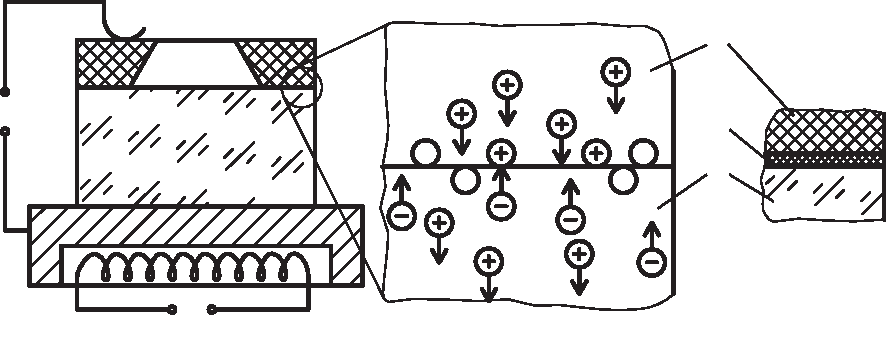
\includegraphics[width=\unitlength]{AB_proc_scheme}}%
        \put(0.01971018,0.28819333){\color[named]{black}\makebox(0,0)[lb]{\smash{$+$}}}%
        \put(0.02175197,0.24680058){\color[named]{black}\makebox(0,0)[lb]{\smash{$-$}}}%
        \put(0.21694339,0.041859){\color[named]{black}\makebox(0,0)[b]{\smash{$\sim$}}}%
        \put(0.21694339,0.00046624){\color[named]{black}\makebox(0,0)[b]{\smash{\textit{а}}}}%
        \put(0.59324114,0.00046624){\color[named]{black}\makebox(0,0)[b]{\smash{\textit{б}}}}%
        \put(0.93567212,0.00046624){\color[named]{black}\makebox(0,0)[b]{\smash{\textit{в}}}}%
        \put(0.81149385,0.19237811){\color[named]{black}\makebox(0,0)[b]{\smash{\textsl{3}}}}%
        \put(0.81149385,0.2450598){\color[named]{black}\makebox(0,0)[b]{\smash{\textsl{2}}}}%
        \put(0.81149385,0.33913425){\color[named]{black}\makebox(0,0)[b]{\smash{\textsl{1}}}}%
        \put(0.4803518,0.248){\color[named]{black}\makebox(0,0)[b]{\smash{SiO\textsubscript{2}}}}%
        \put(0.58571518,0.33160829){\color[named]{black}\makebox(0,0)[b]{\smash{Si${}^{4+}$}}}%
        \put(0.54055945,0.12464451){\color[named]{black}\makebox(0,0)[lb]{\smash{Na${}^+$}}}%
        \put(0.66,0.155){\color[named]{black}\makebox(0,0)[lb]{\smash{O${}^{2-}$}}}%
      \end{picture}%
    \endgroup%

    \caption{Иллюстрация процесса электростатического соединения~\cite{Sinev_osoben_primen_inzh_vest201408}:%
    }
    \label{fig:AB_proc_scheme}
    \textit{а} "--- схема подведения разности потенциалов;
    \textit{б} "--- схема ионного взаимодействия во~время проведения процесса;
    \textit{в} "--- область соединения после завершения процесса.
    \textsl{1} "--- кремний (Si),
    \textsl{2} "--- оксид кремния (SiO\textsubscript{2}),
    \textsl{3}~---~стекло
\end{figure}

\subsection{Основные параметры процесса}
Температура процесса выбирается в~пределах от 180 до 500~{\textdegree}C~\cites[484]{lit_madou2002fundamentals}.
Нижний предел температуры определяется началом ионной проводимости
и~возникновения поляризационных процессов в~стекле.
Верхний предел "--- точкой размягчения стекла
и~температурой плавления материалов топологии на~кремниевом элементе или пластине.
Снижения температуры электростатического соединения можно достичь уменьшением шероховатости поверхности соединяемых материалов, увеличением времени процесса и~прикладываемого электрического напряжения,
а~также применением легкоплавких стёкол с~повышенным содержанием оксида натрия (от 5 до 7~\%).

Прикладываемое электрическое напряжение для электростатического соединения выбирается в~интервале от 200 до 1500~В. Электрическое напряжение можно уменьшить, используя менее шероховатые поверхности, увеличивая температуру и~время выдержки. Верхний предел напряжения ограничивается появлением поверхностных разрядов. Обычно используют источники постоянного или импульсного напряжения. Применения источников переменного напряжения рекомендовано избегать~\cite{Anthony_AB_of_imperfect_surfaces}, поскольку это повышает требования к~шероховатости поверхностей и~к усилию прижатия.

Время процесса электростатического соединения изменяется в~интервале от 1 до 30 мин. Электростатическое соединение осуществляется за~очень короткий промежуток времени, однако, выдержка до~30 минут
повышает прочность соединения.
В~\cite{Rongyan2006Investigation_bond_time} предложена модель оценки
времени требуемого для проведения процесса анодной посадки.

Повышение уровня прилагаемого напряжения снижает длительность процесса~\cite{Lee_Detailed_characterization}. Также время проведения процесса зависит от~характеристик соединяемых пластин и~их покрытий. Необходимое время посадки в~порядке возрастания Si~(p\nb-тип) {\textless} поликремний {\textless} Si\textsubscript{3}N\textsubscript{4} {\textless} SiO\textsubscript{2} {\textless} Si~(n\nb-тип). Si\textsubscript{3}N\textsubscript{4} и~SiO\textsubscript{2} "--- диэлектрические материалы, которые препятствуют дрейфу положительных зарядов к~поверхности соединения~\cite{Lee_Detailed_characterization}.
Вместо этого заряды накапливаются на~поверхности раздела <<нитрид кремния "--- кремний>>.
Это приводит к~возникновению электростатической силы на~поверхности раздела и~замедляет процесс посадки. Кремний p\nb-типа (легированный бором) обеднён электронами по~сравнению с~кремнием n\nb-типа.
Под воздействием электрического поля положительные заряды скапливаются на~поверхности раздела кремний-стекло и~формируют высокую электростатическую силу способствующую быстрому присоединению.

\subsection{Вывод электрических контактов через область соединения кремния со~стеклом}
В некоторых видах МЭМС возникает необходимость вывода электрического контакта через зону соединения кремния и стекла (например, подведение электропитания, шин данных в герметичную область)~\cite{Vacuum_Packaging_Technology_and_Appl}. Это можно сделать несколькими способами, у каждого из которых есть свои преимущества и недостатки, описанные в таких работах как~\cite{Jakobsen_AB_for_MEMS_2001_ppt,tanaka2007laterally,Babaevskij_el_vyvody_NMST2014_4,barinov2015_datchik_zhestk}. Рассмотрим некоторые способы.

В первом из рассматриваемых способов (см. Рисунок \ref{fig:contact_through}а)
на поверхности стекла или кремния вытравливают углубления, в которых затем формируют металлические дорожки. Защитив тем или иным способом дорожки от~электрического контакта с противоположной деталью, осуществляют соединение. К~преимуществам таких токоподводов относят их низкое сопротивление, однако, без дополнительных операций сложно добиться герметичности соединения, а~также есть опасность повреждения дорожек во время соединения. Большое значение для герметичности соединения имеет величина отклонения толщины нанесённого металла от номинала.
\begin{figure}[ht]
    \centering
    \begingroup%
      \makeatletter%
      \providecommand\color[2][]{%
        \errmessage{(Inkscape) Color is used for the text in Inkscape, but the package 'color.sty' is not loaded}%
        \renewcommand\color[2][]{}%
      }%
      \providecommand\transparent[1]{%
        \errmessage{(Inkscape) Transparency is used (non-zero) for the text in Inkscape, but the package 'transparent.sty' is not loaded}%
        \renewcommand\transparent[1]{}%
      }%
      \providecommand\rotatebox[2]{#2}%
      \ifx\svgwidth\undefined%
        \setlength{\unitlength}{424.91000018bp}%
        \ifx\svgscale\undefined%
          \relax%
        \else%
          \setlength{\unitlength}{\unitlength * \real{\svgscale}}%
        \fi%
      \else%
        \setlength{\unitlength}{\svgwidth}%
      \fi%
      \global\let\svgwidth\undefined%
      \global\let\svgscale\undefined%
      \makeatother%
      \begin{picture}(1,0.74055627)(0,-0.048206627878)
        \put(0,0){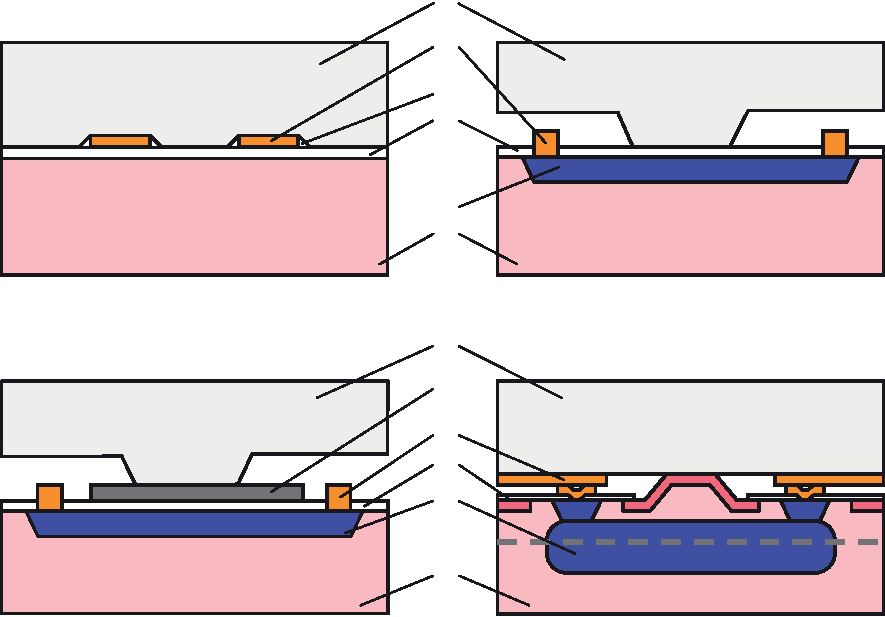
\includegraphics[width=\unitlength]{contact_through.pdf}}%
        \put(0.49600326,0.67879616){\color[named]{black}\makebox(0,0)[lb]{\smash{\textsl{1}}}}%
        \put(0.49535263,0.63262167){\color[named]{black}\makebox(0,0)[lb]{\smash{\textsl{4}}}}%
        \put(0.49590687,0.41855278){\color[named]{black}\makebox(0,0)[lb]{\smash{\textsl{2}}}}%
        \put(0.49422532,0.45145387){\color[named]{black}\makebox(0,0)[lb]{\smash{\textsl{6}}}}%
        \put(0.4958667,0.54705054){\color[named]{black}\makebox(0,0)[lb]{\smash{\textsl{3}}}}%
        \put(0.49540884,0.57670397){\color[named]{black}\makebox(0,0)[lb]{\smash{\textsl{5}}}}%
        \put(0.49600326,0.29330271){\color[named]{black}\makebox(0,0)[lb]{\smash{\textsl{1}}}}%
        \put(0.49535263,0.19445824){\color[named]{black}\makebox(0,0)[lb]{\smash{\textsl{4}}}}%
        \put(0.49590685,0.03305937){\color[named]{black}\makebox(0,0)[lb]{\smash{\textsl{2}}}}%
        \put(0.49422532,0.11863041){\color[named]{black}\makebox(0,0)[lb]{\smash{\textsl{6}}}}%
        \put(0.49585521,0.16155713){\color[named]{black}\makebox(0,0)[lb]{\smash{\textsl{3}}}}%
        \put(0.49340073,0.24388048){\color[named]{black}\makebox(0,0)[lb]{\smash{\textsl{7}}}}%
        \put(0.2105012,0.34332804){\color[named]{black}\makebox(0,0)[lb]{\smash{\textit{а}}}}%
        \put(0.21022771,-0.03905968){\color[named]{black}\makebox(0,0)[lb]{\smash{\textit{в}}}}%
        \put(0.76944963,0.34332804){\color[named]{black}\makebox(0,0)[lb]{\smash{\textit{б}}}}%
        \put(0.77107451,-0.03905968){\color[named]{black}\makebox(0,0)[lb]{\smash{\textit{г}}}}%
      \end{picture}%
    \endgroup%

    \caption{Схематическое изображение способов вывода электрических контактов через область соединения~\cite{Jakobsen_AB_for_MEMS_2001_ppt}:}
    \label{fig:contact_through}
    \textit{а} "--- вытравливанием каналов под проводники; \textit{б} "--- диффузионный <<приповерхностный>> проводник; \textit{в} "--- соединение с~плёнкой поликристаллического кремния; \textit{г} "--- заглублённый диффузионный проводник. \textsl{1} "--- стекло, \textsl{2} "--- кремний (Si), \textsl{3} "--- оксид кремния (SiO\textsubscript{2}),
    \textsl{4}~---~металлизация;
    \textsl{5}~---~вытравленный канал; \textsl{6} "--- легированный кремний (проводимость p+);
    \textsl{7}~---~слой поликристаллического кремния
\end{figure}

Следующий способ (см. Рисунок \ref{fig:contact_through}б) заключается в легировании приповерхностной области кремния с нанесением металлизации в областях будущей разварки и защите оксидом в остальных местах. Этот способ сохраняет герметичность последующего соединения, однако, сопротивление токопровода заметно выше, чем в предыдущем варианте. Кроме того, на ионных взаимодействиях в~процессе соединения отрицательно сказывается наличие легированной области. Снизить негативные последствия возможно осаждением в~области соединения поверх оксида слоя поликристаллического кремния  (см. Рисунок \ref{fig:contact_through}в),
на~который затем производят электростатическое присоединение стекла.

В следующем способе (см. Рисунок \ref{fig:contact_through}г) после легирования приповерхностной
области осуществляют эпитаксиальное наращивание слоя кремния. Таким образом, проводящая область
оказывается заглублена в месте будущего соединения. Токоподвод к ней осуществляют через области ещё
одного легирования, которые обеспечивают её связь с поверхностью.

Металлические дорожки толщиной более 0,2 мкм препятствуют плотному контакту соединяемых пластин, необходимому для качественного соединения поверхностей~\cite{Cozma_Puers_1995}. Толщина дорожек SiO\textsubscript{2} свыше 0,3 мкм также препятствует плотному контакту~\cite{Cozma_Puers_1995}.

\subsection{Моделирование изменения тока в процессе соединения}

Для предсказания экспериментального поведения тока в зависимости от~времени начиная с 1970-х годов предпринимаются попытки сформировать достаточно точную теоретическую модель.

В работе~\cite{Carlson1972polarization}
были предприняты попытки моделирования долговременного поведения тока. В этой модели для ионов была введена мобильность, зависящая от поля, и было сделано предположение, что всё падение напряжения происходит в слое отрицательного заряда в стекле.

В модели эквивалентной электрической цепи по~\cite{Anthony_AB_of_imperfect_surfaces} (Рисунок~\ref{fig:process_model}), слой пространственного заряда заменён постоянной емкостью, вызывающей экспоненциальное затухание тока. Эту модель используют для оценки зависимости электростатических сил, стягивающих соединяемые образцы, от~приложенного напряжения, и зависимости тока от времени. Здесь: R\textsubscript{1} "--- последовательное сопротивление стекла; R\textsubscript{2} "--- сопротивление утечки; C "--- ёмкость соединяемой пары; V "--- приложенная разность потенциалов. Определив заряд конденсатора в~модели, можно определить получаемую силу притягивания соединяемых деталей.
\begin{figure}[ht]
    \centering
    \begingroup%
      \makeatletter%
      \providecommand\color[2][]{%
        \errmessage{(Inkscape) Color is used for the text in Inkscape, but the package 'color.sty' is not loaded}%
        \renewcommand\color[2][]{}%
      }%
      \providecommand\transparent[1]{%
        \errmessage{(Inkscape) Transparency is used (non-zero) for the text in Inkscape, but the package 'transparent.sty' is not loaded}%
        \renewcommand\transparent[1]{}%
      }%
      \providecommand\rotatebox[2]{#2}%
      \ifx\svgwidth\undefined%
        \setlength{\unitlength}{120.24470172bp}%
        \ifx\svgscale\undefined%
          \relax%
        \else%
          \setlength{\unitlength}{\unitlength * \real{\svgscale}}%
        \fi%
      \else%
        \setlength{\unitlength}{\svgwidth}%
      \fi%
      \global\let\svgwidth\undefined%
      \global\let\svgscale\undefined%
      \makeatother%
      \begin{picture}(1,1.67141667)%
        \put(0,0){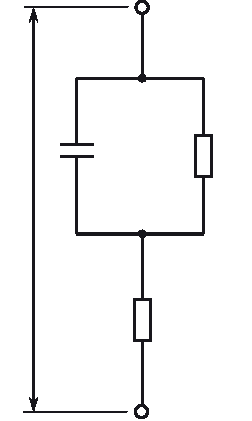
\includegraphics[width=\unitlength]{process_model.pdf}}%
        \put(0.6251985,0.3569699){\color[named]{black}\makebox(0,0)[lb]{\smash{R\textsubscript{1}}}}%
        \put(0.86870192,1.00914014){\color[named]{black}\makebox(0,0)[lb]{\smash{R\textsubscript{2}}}}%
        \put(0.39616544,1.03413581){\color[named]{black}\makebox(0,0)[lb]{\smash{C}}}%
        \put(-0.00102444,0.79774986){\color[named]{black}\makebox(0,0)[lb]{\smash{V}}}%
      \end{picture}%
    \endgroup%
    \caption{Модель эквивалентной электрической цепи процесса электростатического соединения~\cite{Anthony_AB_of_imperfect_surfaces}}
    \label{fig:process_model}
\end{figure}

Автор работы~\cite{Albaugh1991electrode_phenomena}
указал, что эти модели не годятся для начального промежутка времени, когда падение напряжения в стекле происходит из-за сопротивления стекла, а не ёмкости области пространственного заряда. Он~создал модель, которая включает граничные условия для начального промежутка времени, и получил качественное соответствие с экспериментальной зависимостью тока от времени. Когда его уравнения выводятся из экспериментальных характеристик материалов, его модель имеет значительные расхождения с соответствующими экспериментальными результатами~\cite{Rios2000_modelling_current}.

В работе~\cite{Rios2000_modelling_current} была представлена модель, сформулированная на основе изменений во времени слоёв в стекле, обеднённых катионами и анионами.
Аналитическое решение учитывает как кратковременный рост тока, так и~долговременное экспоненциальное падение тока. Переход между двумя режимами происходит, когда электрическое поле на стыке кремния со стеклом достигает величины достаточной для дрейфа анионов~\cite{Rios2000_modelling_current}.

В работе~\cite{Anthony_AB_of_imperfect_surfaces} все элементы эквивалентной электрической схемы (Рисунок~\ref{fig:process_model}) считаются постоянными во времени. В работе~\cite{He2015_electric_curr_charact} при той же схеме все её элементы считаются переменными во времени. Также в работе~\cite{He2015_electric_curr_charact} учитывается площадь плотного контакта, а полные заряды перемещённых ионов щелочных металлов и электрического поля считаются различающимися величинами. В этой модели: R\textsubscript{1} "--- сопротивление стекла и катодного контакта (заметную роль играет размер катода, точечный или же конечной площади); R\textsubscript{2} "--- сопротивление слоя обеднённого щелочными ионами, в связи с переменной толщиной слоя, также является переменным; C "--- ёмкость слоя обеднённого щелочными ионами, рассчитываемая с учётом эквивалентной площади плотного контакта и толщины слоя обеднённого щелочными ионами.

\subsection{Борьба с~локальным перегревом стыка материалов}\label{chap:local_heating}

Наиболее часто процесс электростатического соединения проводят при постоянном напряжении, однако, в этом случае начальный скачок тока может вызывать локальный перегрев поверхностей и привести к большим остаточным напряжениям~\cite{Sinev_osoben_primen_inzh_vest201408}.
Во избежание такого эффекта применяют ограничение по~току~\cite{Rogers_current_limited_AB_2005}.
В течение процесса поддерживают относительно низкое значение тока за счёт плавного роста напряжения.
Это снижает риск локального перегрева поверхностей, но в то же время может увеличить длительность процесса.

Пиковые значения тока при соединении пластин диаметром 100~мм могут достигать нескольких десятков миллиампер, что, в случае подачи разницы потенциалов в 1~кВ, говорит о рассеянии нескольких десятков ватт тепла~\cite{Rogers_current_limited_AB_2005}.

Однако из-за неидеальной плоскостности поверхностей, кремний и стекло будут соприкасаться лишь в некоторых точках, через которые станет протекать ток. Протекание тока, в соответствии с законом Джоуля"--~Ленца, может вызвать локальный нагрев частей стыка до температур выше предполагаемых по показаниям термодатчиков на электродах. Различие в локальных температурах на~стыке кремния со стеклом в момент их соединения может вызвать локальные вариации остаточных напряжений при охлаждении до~рабочих температур~\cite{Rogers_current_limited_AB_2005}.

При проведении процесса с~ограничением тока, подводимое напряжение
изначально очень низкое и~затем постепенно возрастает с~увеличением
соединённой площади пластин. При таком режиме происходит лучшее
управление температурой стыка и её воспроизводимостью от процесса к
процессу~\cite{Rogers_current_limited_AB_2005}.

\subsection{Анализ прочности получаемого соединения}
Дать характеристику проходящему или уже завершившемуся процессу можно
несколькими способами: наблюдением за параметрами процесса (за током),
визуальным осмотром (область соединения имеет более тёмный оттенок
серого цвета в отличие от несоединённых областей), проводя разрушающие
испытания на отрыв или сдвиг, измеряя изгиб соединённых деталей.
Механическая прочность соединения составляет от 10 до
150~МПа~\cite{guan2006icept06,
Hu2008tensile_tests,
Villanueva2006_Transfer_small}. Величина прочности зависит от
материалов и метода измерения. Обычно соединённые детали разрушаются с
вырывом кремния, либо стекла~\cite{Khomenko1982useglassproperties}. К
дефектам соединения относят: пустоты из-за посторонних частиц,
несоединённые области из-за неплоскостности соединяемых поверхностей,
погрешности совмещения.

В~\cite{Cozma_Puers_1995} было отмечено повышение твёрдости стекла вследствие миграции ионов и предложено снижать этот эффект применением точечного электрода.

Механизмы различных методов соединения были подробно объяснены к~настоящему времени, но методы для оценки соединения должны разрабатываться постоянно с развитием технологии микрообработки в более сложные структуры с высокими требованиями по надёжности~\cite{Richard2002weibull_fracture_probability}. Метод, описанный в~работе~\cite{Maszara1988bonding_silicon}, заключается в введении тонкого лезвия в область соединения и~последующем вычислении энергии поверхности исходя из обследования разлома на кончике лезвия. Этот метод легко применим, но ограничен слабыми соединениями. Когда анодная посадка формирует прочные соединения и,~более того, использует как одну из составных частей хрупкий материал "--- стекло, метод лезвия не подходит. Метод растягивающего или трёхточечного изгиба неудобен в~применении и неэффективен при отражении связи прочности соединения с~условиями соединения~\cite{Richard2002weibull_fracture_probability}. При изучении влияния параметров процесса соединения на качество соединения, были разработаны оптические и неразрушающие методы~\cite{Go1999Experimental_eval_Taguchi, TaticLucic1997bond_characterization, Plaza1997nondestructive}. Они легки в применении и позволяют оценить электростатическое давление во время анодной посадки~\cite{Richard2002weibull_fracture_probability}, хотя ещё остаётся в~силе вопрос, можно ли эти методы соотнести с реальной прочностью соединения~\cite{TaticLucic1997bond_characterization}. Известен микрошевронный тест для оценки прочности соединённых пластин кремния~\cite{Petzold1999quality_reliability_chevron}. Этот метод можно использовать и для анодной посадки~\cite{Richard2002weibull_fracture_probability}.

Всё ещё существует необходимость в методах оценки для определения надёжности соединённых микроструктур. Ранее описанные испытания растягивающим изгибом показали, что трещины обычно инициируются на стыке кремний-стекло, но распространяются по стеклу. Из этого был сделан вывод, что именно прочность стыка определяет надёжность всего прибора~\cite{Richard2002weibull_fracture_probability}. В работе~\cite{Richard2002weibull_fracture_probability} описаны испытания прочности стыка посредством подачи газа под давлением и~дальнейший статистический анализ с применением распределения Вейбулла.

\subsection{Формирование гребенчатых структур в системе «кремний на~стекле»}
В случае проведения электростатического соединения кремния со стеклом в вакууме возможен изгиб мембраны над полостью в кремнии. Если на~этих мембранах в дальнейшем будут производиться литографические операции, то~возможно искажение формы получаемых элементов. Это относится, например, к~гребенчатым структурам.

Существует проблема повреждений высокоаспектных гребенчатых структур во время их формирования глубинным плазмохимическим травлением над таким диэлектриком как стекло. Детальное описание проблемы и~возможное решение в виде формирования дополнительной металлической плёнки на стекле описано в~\cite{LeeMC2005_gyro_siog}. В этих работах показано, что введение стадии напыления плёнки металла перед операцией освобождения гребёнки чувствительного элемента позволяет резко увеличить коэффициента выхода годных приборов.

\subsection{Предотвращение нежелательного соединения}\label{chap:unintentional_bond}
При применении анодной посадки для соединения деталей с подвижными
элементами есть опасность того, что из-за сильного электростатического
поля гибкая структура притянется к стеклу и соединится
с~ним~\cite{Cozma_Puers_1995}. Нужно использовать как конструктивные,
так и технологические решения, которые бы~предотвратили контакт
кремния со стеклом в нежелательных
областях~\cite{Yu2008_Yield_improvement_AB}.
Для решения этой задачи есть несколько вариантов:
\begin{itemize}
    \item понижение подводимой разности потенциалов, чтобы снизить стягивающие электростатические силы;
    \item экранирование мест соединения~\cite{lit_Esashi_Wafer2008};
    \item локальная модификация поверхности с~целью препятствования соединению~\cites[6]{ushkov2008_avtoref}.
\end{itemize}

\section{Следствия тепловой несогласованности кремния и стекла}\label{chap_temp_inconsistence}
В результате соединения образуются остаточные напряжения.
Напряжения, возникающие вследствие разности ТКЛР стекла и кремния называют
коэффициентными напряжениями~\cite{ost_Steklo_terminy}. Также, механические
напряжения, возникающие в результате различия ТКЛР соединяемых материалов после
их охлаждения, называют термическими~\cites[С.~19, 26]{mehan_napr_plenki1981obzor}.
До начала нагрева стеклянная и кремниевая детали имеют одинаковые размеры, при
нагреве детали расширяются неравномерно и~при~температуре соединения $T_b$ имеют
отличающиеся размеры. После соединения детали, охлаждаясь до рабочей температуры
$T_w$, взаимно деформируются~\cite{Sinev_Ryabov_rasch_coef_napr_nmst2014}.
В работе~\cites[13]{matuzov2008_avtoref} говорится, что <<для плоских
мембран чувствительность уменьшается с~увеличением значения внутренних
напряжений>>.
Cогласно~\cite{Cozma_Puers_1995} формирующиеся после
соединения механические напряжения в~стекле являются важным критерием
оптимизации режима процесса анодной посадки.

Наглядно деформации выражаются в прогибе соединённых пластин.
В~работе~\cite{Rogers1992considerations} говорится о прогибе порядка 30~мкм
даже когда кремний соединён со~стеклом толщиной 3~мм.
В работе~\cite{rogers1995selection} говорится о прогибе 100~мкм в~случае
соединения пластин кремния с пластинами стекла Corning~7070 толщиной 1~мм
при 460~{\textdegree}C.
В~\cite{Rogers_current_limited_AB_2005} выдвинуто требование прогиба не
более 70~мкм для производства микрогироскопов.
В работе~\cite{LeeMC2005_gyro_siog} говорится о прогибе до~110~мкм
в~случае соединения пластин кремния толщиной 500~мкм с~пластинами стекла
Corning~7740 толщиной 350~мкм при 460~{\textdegree}C.

Согласно~\cite{Rogers1992considerations, rogers1995selection} прогиб
пластины стекла также может быть вызван изменением распределения её состава
по толщине вследствие дрейфа ионов.
В~\cite{Sadaba2006CompositionalGradients} проведено
исследование влияния смоделированной неравномерности распределения состава
также и по площади пластины вследствие применения как точечного, так
и плоского электродов.
В~\cite{Rogers1992considerations} предлагается снижать возникающий прогиб
пластин подведением по завершении соединения тока обратной полярности для
изменения стехиометрии стекла или же проводить процесс соединения так,
чтобы в момент соединения пластины кремния и~стекла имели разные,
специально подобранные температуры. Второй из этих подходов был подробно проверен в работе~\cite{Inzinga2012_infrared_characterization}.

В~\cite{maj2014influence_proceedings} показано средствами конечно-элементного моделирования, что сборка чувствительного элемента датчика давления в оптимальных условиях из~\cite{ettouhami1996thermal} даёт разброс механических напряжений не~менее 10~\% в~мембране, работающей в~интервале температур от~0~до~50~{\textdegree}C.

В работе~\cite{Kim2015warpage} описаны различные способы оценки остаточных напряжений,
возникающих в стекле, соединяемом с кремнием, с учётом исследований вязкости
и моделей вязкоупругости материалов.
В ней разработаны модели оценки остаточных напряжений и возникающего прогиба пластин, которые могут учитывать термообработку в виде выдержки соединённых деталей в~течение нескольких часов при температурах от 450 до 560~{\textdegree}C.
Также рассмотрено влияние скорости охлаждения на температуру стеклования. Рассчитана возможность управления прогибом пластин за счёт подобной термообработки. Практические эксперименты в этой области были описаны ранее в работе~\cite{Harz1996Curvature_changing}, и~некоторые реализации были запатентованы в~\cite{engelke1998process_bend_patent} (в настоящее время патент не~поддерживается).

В~\cite{Cozma_Puers_1995} были представлены результаты измерений деформаций при разных температурах соединения. Было показано, что с ростом температуры, растут и~деформации. Также там же было показано, что чем толще стеклянная пластина, тем больше вызываемые механические напряжения в кремнии. В~зависимости от толщины стекла температура ненапряженного соединения находится в интервале от 265 до 315~{\textdegree}C~\cite{Cozma_Puers_1995}. В~\cite{ettouhami1996thermal} было заявлено, что оптимальная температура посадки с пирексом 270~{\textdegree}C. В связи с этим, в целях минимизации последствий различия ТКЛР электростатическое соединение кремния со~стеклом
стараются проводить при температурах около 300~{\textdegree}C~\cite{Low_temp_wafer_AB}.

Существует температура, при которой формируется соединение, не вызывающее механических напряжений~\cite{Cozma_Puers_1995}. В зависимости от температуры соединения можно получить сжимающие напряжения или растягивающие напряжения~\cite{Cozma_Puers_1995}. При сжимающих напряжениях, их носитель стремится расшириться, при растягивающих напряжениях "--- сжаться~\cites[19]{mehan_napr_plenki1981obzor}. Растягивающие напряжения считают положительными, сжимающие "--- отрицательными~\cites[5]{mehan_napr_plenki1981obzor}.

Снижение температуры электростатического соединения требует повышения прилагаемой разности потенциалов, поскольку в связи со снижением мобильности ионов, требуется большее усилие для их смещения~\cite{Low_temp_wafer_AB, Cozma_Puers_1995}.

\section{Постановка цели и~задач исследования}

\providecommand{\beforenedostati}%
{Несмотря на~большое количество исследований применения технологии
электростатического соединения кремния со~стеклом,
ряд вопросов остаётся невыясненным.
С повышением требований к~электронным приборам возросли требования
к минимизации остаточных напряжений.
}

\providecommand{\beforenedostatii}%
{Среди вопросов, остающихся нерешёнными,
стоит отметить следующие:}

\providecommand{\nedostati}% %с большой буквы и без точки в конце
{Недостаточно данных по~термомеханическим свойствам стёкол, подходящих
для электростатического соединения с кремнием, в форме, удобной
к применению в аналитических расчётах и в~системах компьютерного
моделирования}

\providecommand{\nedostatii}% %с большой буквы и без точки в конце
{Недостаточно хорошо исследован выбор температуры соединения
и~предпосылки наличия температуры проведения соединения
с минимальными остаточными напряжениями}

\providecommand{\nedostatiii}% %с большой буквы и без точки в конце
{Недостаточно подробно описано влияние соотношения толщин
соединяемых пластин на~возникающие после соединения напряжения}
%
\beforenedostati{}
\beforenedostatii{}
\begin{enumerate}
    \item \nedostati{}.
    \item \nedostatii{}.
    \item \nedostatiii{}.
\end{enumerate}

На основании вышесказанного с целью
\MakeLowercase{\protect\aimTextContentRod{}}
задачи исследования можно сформулировать следующим образом:
\begin{enumerate}
\item \label{task1}\mmark{Исследовать зависимость} температурных коэффициентов линейного расширения
(\mmark{ТКЛР}) \mmark{от~температуры для стёкол}, совместимых с~анодной посадкой.
\item \label{task2}\mmark{Разработать модели оценки} остаточных напряжений, определить
их~возможности по учёту температурной зависимости ТКЛР, распределению
напряжений по~толщине материалов и~подбору температуры соединения
с~минимальными остаточными напряжениями.
\item \label{task3}\mmark{Разработать методику расчёта} остаточных напряжений
при использовании известных марок стёкол.
\item \label{task4}\mmark{Предложить способ коррекции} температуры
и~выбора толщины соединяемых деталей, обеспечивающих
минимальную величину остаточных напряжений.
\item \label{task5}Разработать методику и~\mmark{провести экспериментальные
исследования} процесса соединения кремния со~стеклом с~измерением
остаточных напряжений в~соединении.

\end{enumerate}
